
\subsection{凸包法}
\label{subsec:lab4-convex-hull}

\paragraph{基本原理}

首先先介绍一下凸包

凸集，就是集合中任意两点之间的线段都完全属于这个集合：
\[
\forall x,y\in C,\ \forall \lambda\in[0,1],\quad
\lambda x+(1-\lambda)y\in C
\]
对有限集合 \(P\)，它的凸包 \(\operatorname{conv}(P)\) 是\(\mathbb{R}^n\)中包含 \(P\) 的最小凸集

那么也就是说，凸包其实就是把集合里的点都连起来，然后把扫过的所有区域都包含进来

那前面的one-hot方法有一个问题就是变量太多了，每个点都要一个

那就和前面逻辑化简类似，我们尽可能把能合并的合并

那凸包就是包含一个点集的最小凸集。对于有限个点来说，凸包就可以把这个集合全部囊括

凸包还包含点之间的连续区域；只有再要求$x\in\{0,1\}^8$，才能用后文的性质保证可行点仍属于原点集
\begin{figure}[H]
    \centering
    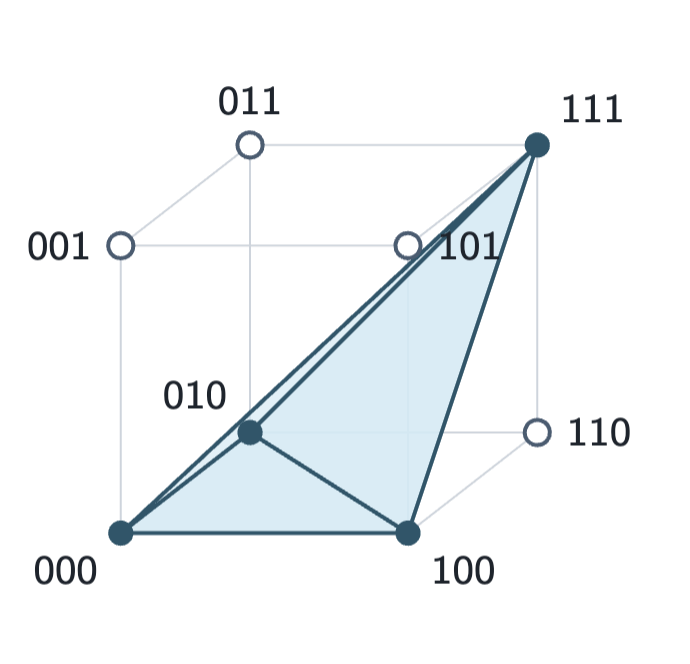
\includegraphics[width=0.5\textwidth]{figures/convex.png}
\end{figure}
从直觉来看，我们把边缘的点连成凸多边形就能变成凸包，因为把所有点都包住了，也就是说边界都是像图中的直线

那我们毕竟也不是数学系，这个就不证明了

凸多边形在高维叫多胞体，可以通过有限个线性不等式和等式来描述，这种表示方法就称为H表示

可以写成
\[
P=\{x\in\mathbb R^8\mid Ax+b\ge0,\ Cx+d=0\}.
\]

其中$A$和$b$分别表示不等式的系数矩阵和常数向量，$C$和$d$则表示等式的系数矩阵和常数向量。

因此，我们只需要将这些系数整理成矩阵形式，就可以得到完整的凸包模型：
\begin{equation}
\begin{aligned}
\min\quad &0\\
\text{s.t.}\quad
&Ax+b\ge0,\\
&Cx+d=0,\\
&x\in\{0,1\}^8.
\end{aligned}
\label{eq:lab4-full-hull-model}
\end{equation}


\paragraph{正确性分析}

首先，对于任意可达点$x\in V$，根据凸包的定义，显然有$x\in P$,所以不会漏点

不过这里有一个问题：凸包中除了原来的可达点，还会包含这些点之间的连续区域，那会不会引入新的点呢

假设存在$x\in P$，$V=\{v^{(1)},v^{(2)},...\}$

那么根据凸包的定义，存在一组非负实数$\theta_i$，使得
\[
x=\sum_{i=1}^{N}\theta_i v^{(i)},
\qquad
\theta_i\ge0,\quad
\sum_{i=1}^{N}\theta_i=1.
\]

由于$x$和$v^{(i)}$的每个坐标都只能取0或1

如果$x_j=0$，那么
\[
0=\sum_{i=1}^{N}\theta_i v_j^{(i)}.
\]

由于每一项都非负，所以对所有$\theta_i>0$的项，必有$v_j^{(i)}=0$

同理，如果$x_j=1$，那么
\[
1=\sum_{i=1}^{N}\theta_i v_j^{(i)}.
\]

因为所有$v_j^{(i)}\le1$，而$\theta_i$非负且和为1，所以对所有$\theta_i>0$的项，必有$v_j^{(i)}=1$

因此任取一个$\theta_i>0$的项，均有$x=v^{(i)}$

因此，$x$本身必然就是$V$中的某个点，不会产生新的点

综上，
\[
P\cap\{0,1\}^{8}=V.
\]

也就是说$\text{conv}(V)\cap\{0,1\}^{8}=V$

正是这个性质才让我们把$(a,b)$编码成bit,因为你如果是单纯的整数的话，就没有这么好的性质了
\paragraph{基于不可达点覆盖的贪心筛选}

那我们的H表示可能依旧得到很多不等式，我们也需要合并化简

这里我们可以采用贪心算法

假设凸包的H表示为
\[
Ax+b\ge0,\qquad Cx+d=0.
\]

对于其中第$i$条不等式，我们记为
\[
A_i x+b_i\ge0,
\]

如果某个不可达点$q\in Q$满足
\[
A_iq+b_i<0,
\]

因此，我们可以把第$i$条不等式能够排除的全部不可达点记为
\[
R_i=\{q\in Q\mid A_iq+b_i<0\}.
\]

这样，每条不等式都对应一个不可达点集合

而我们希望从这些集合中选出尽可能少的几个，使它们能够覆盖全部不可达点，那就只需要这么几个不等式就够了

这实际上就是一个集合覆盖问题。

不过需要注意，H表示中除了不等式，还可能包含等式

由于等式约束需要保留，因此那些已经违反等式的不可达点，就没有必要再通过不等式排除

我们可以先将满足
\[
Cq+d\ne0
\]
的不可达点从$Q$中删除。

剩下的不可达点记为
\[
Q_{\mathrm{remaining}}.
\]

接下来，我们每次从尚未选中的不等式中，找出能够排除最多剩余不可达点的那一条。

具体来说，选择
\[
i^*=\underset{i\in\mathrm{pool}}{\operatorname{arg\,max}}
\left|R_i\cap Q_{\mathrm{remaining}}\right|.
\]

其中$\mathrm{pool}$表示尚未选中的候选不等式集合。

选中后，将这条不等式加入保留集合，并更新剩余点集：
\[
Q_{\mathrm{remaining}}
\leftarrow
Q_{\mathrm{remaining}}\setminus R_{i^*}.
\]

然后继续寻找下一条能够排除最多剩余不可达点的不等式。

不断重复这个过程，直到
\[
Q_{\mathrm{remaining}}=\varnothing.
\]

这就说明，所有不可达点都已经被选中的约束排除了

在具体代码实现中，我们可以使用三个列表：

\begin{itemize}
    \item \texttt{remaining}：保存尚未排除的不可达点；
    \item \texttt{pool}：保存尚未选中的候选不等式；
    \item \texttt{chosen}：保存已经选中的不等式。
\end{itemize}

每次从\texttt{pool}中选择能够排除最多剩余点的不等式，将其加入\texttt{chosen}，同时从\texttt{remaining}中删除被它排除的点。

\paragraph{约简模型的正确性分析}

假设经过贪心筛选后，我们得到了保留下来的不等式集合

将这些不等式对应的系数重新组成矩阵$A'$和向量$b'$，那么约简后的模型可以写成
\begin{equation}
\begin{aligned}
\min\quad &0\\
\text{s.t.}\quad
&A'x+b'\ge0,\\
&Cx+d=0,\\
&x\in\{0,1\}^{8}.
\end{aligned}
\label{eq:lab4-reduced-hull-model}
\end{equation}

接下来，我们证明约简后的模型仍然成立

首先，所有保留下来的约束都来自原来的完整H表示

由于所有可达点都满足完整H表示，那么删除其中一部分不等式之后，可达点自然仍然满足剩下的约束

反过来，对于任意不可达点$q\in Q$，我们分两种情况讨论

如果$q$不满足等式约束
\[
Cq+d=0,
\]
那么它已经被等式排除，不可能成为模型的可行解

如果$q$满足全部等式约束，那么它就属于贪心算法初始时尚未排除的点集

由于贪心算法只有在所有剩余不可达点都被排除之后才会结束，因此必然存在某条被保留的不等式，使得
\[
A'_iq+b'_i<0.
\]

所以$q$同样不满足约简后的模型。

这说明全部不可达点都被排除

当然贪心算法求出来的不一定是最优解，不过我们也实现了减少约束数量的目的

最后，对于差分传播和线性传播，我们分别利用DDT和LAT中的非零位置构造可达点集，再独立计算凸包并进行约束筛选
